% File: solutions/ex16.tex

\begin{soluzione}{16}
    Questo esercizio illustra come rappresentare lo spettro di un segnale campionato sia in termini di frequenza assoluta ($f$ in Hz) sia in termini di frequenza normalizzata ($\nu$), che è adimensionale.

    \subsubsection*{Dati del problema}
    \begin{itemize}
        \item Spettro originale: $X(f) = \text{rect}\left(\frac{f}{200}\right)$. Questo è un rettangolo di ampiezza 1 che si estende da -100 Hz a 100 Hz. La banda del segnale è $B=100$ Hz.
        \item Frequenza di campionamento: $f_s = 150$ Hz.
    \end{itemize}
    Come nell'Esercizio 6, la condizione di Nyquist ($f_s \ge 2B$) è violata, quindi si verifica aliasing.

    \begin{enumerate}
        \item \textbf{Spettro campionato in funzione di $f$ [Hz]}
        
        Lo spettro campionato $\tilde{X}(f)$ è la somma delle repliche di $X(f)$, scalate per un fattore $1/T = f_s = 150$.
        \begin{itemize}
            \item La replica centrale (k=0) è un rettangolo di altezza 150 da -100 Hz a 100 Hz.
            \item Le repliche adiacenti (k=$\pm 1$) sono centrate a $\pm 150$ Hz.
        \end{itemize}
        A causa dell'aliasing, le repliche si sommano. L'ampiezza di $\tilde{X}(f)$ è:
        \begin{itemize}
            \item $150$ nell'intervallo $|f| < 50$ Hz (solo replica centrale).
            \item $150+150 = 300$ negli intervalli $50 \le |f| < 100$ Hz (sovrapposizione).
        \end{itemize}
        Il grafico di $\tilde{X}(f)$ è il seguente:
        
        \begin{center}
        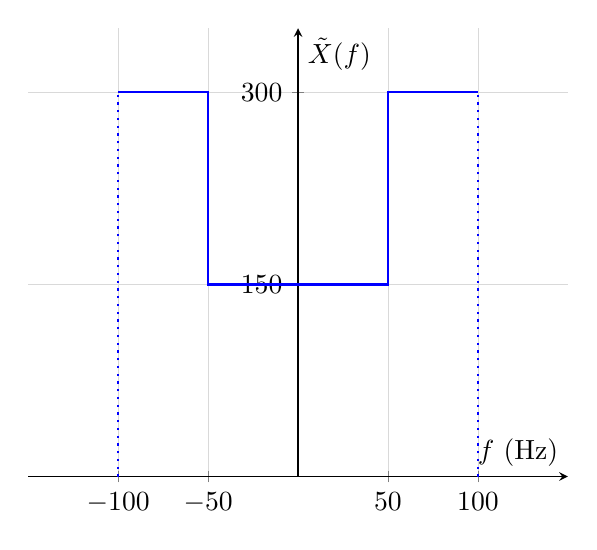
\begin{tikzpicture}
            \begin{axis}[
                axis lines=middle, xlabel=$f$ (Hz), ylabel=$\tilde{X}(f)$,
                xmin=-150, xmax=150, ymin=0, ymax=350,
                xtick={-100, -50, 0, 50, 100}, ytick={150, 300},
                grid=both, grid style={line width=.1pt, draw=gray!30}
            ]
            \addplot[blue, thick] coordinates {
                (-100, 300) (-50, 300) (-50, 150) (50, 150) (50, 300) (100, 300)
            };
            \draw[blue, thick, dotted] (axis cs: -100,0) -- (axis cs:-100,300);
            \draw[blue, thick, dotted] (axis cs: 100,0) -- (axis cs:100,300);
            \end{axis}
        \end{tikzpicture}
        \end{center}

        \item \textbf{Introduzione della frequenza normalizzata $\nu$}
        
        La frequenza normalizzata, spesso indicata con $\nu$ o $\phi$, è una frequenza adimensionale definita come il rapporto tra la frequenza assoluta $f$ e la frequenza di campionamento $f_s$:
        \[
            \mathbf{\nu = \frac{f}{f_s}}
        \]
        Questa variabile misura la frequenza in "cicli per campione" invece che in "cicli per secondo" (Hz). È estremamente utile perché rende l'analisi indipendente dalla specifica $f_s$ utilizzata. L'intervallo di Nyquist in frequenza normalizzata è sempre $[-0.5, 0.5]$.
        
        \item \textbf{Spettro campionato in funzione di $\nu$}
        
        Per ottenere il grafico di $\tilde{X}(\nu)$, semplicemente riscaliamo l'asse delle ascisse del grafico precedente dividendolo per $f_s = 150$ Hz.
        \begin{itemize}
            \item $f = \pm 50 \text{ Hz} \implies \nu = \pm\frac{50}{150} = \pm\frac{1}{3}$
            \item $f = \pm 100 \text{ Hz} \implies \nu = \pm\frac{100}{150} = \pm\frac{2}{3}$
        \end{itemize}
        Il grafico di $\tilde{X}(\nu)$ è identico nella forma, ma con l'asse delle frequenze normalizzato:
        
        \begin{center}
        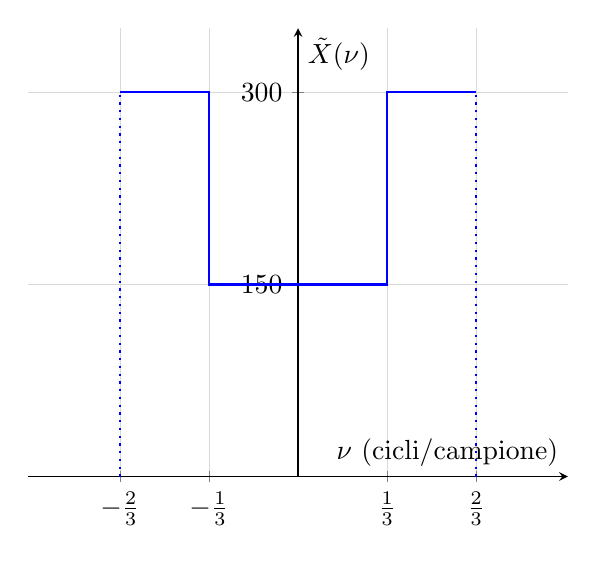
\begin{tikzpicture}
            \begin{axis}[
                axis lines=middle, xlabel=$\nu$ (cicli/campione), ylabel=$\tilde{X}(\nu)$,
                xmin=-1, xmax=1, ymin=0, ymax=350,
                xtick={-0.66, -0.33, 0, 0.33, 0.66},
                xticklabels={$-\frac{2}{3}$, $-\frac{1}{3}$, 0, $\frac{1}{3}$, $\frac{2}{3}$},
                ytick={150, 300},
                grid=both, grid style={line width=.1pt, draw=gray!30}
            ]
            \addplot[blue, thick] coordinates {
                (-0.66, 300) (-0.33, 300) (-0.33, 150) (0.33, 150) (0.33, 300) (0.66, 300)
            };
            \draw[blue, thick, dotted] (axis cs: -0.66,0) -- (axis cs:-0.66,300);
            \draw[blue, thick, dotted] (axis cs: 0.66,0) -- (axis cs:0.66,300);
            \end{axis}
        \end{tikzpicture}
        \end{center}
        
        Nello spazio della frequenza normalizzata, lo spettro di \textit{qualsiasi} segnale campionato è sempre periodico con \textbf{periodo 1}. Questo perché un incremento della frequenza assoluta $f$ di un valore $f_s$ corrisponde a un incremento della frequenza normalizzata $\nu$ di $f_s/f_s = 1$.
        
    \end{enumerate}
\end{soluzione}